\documentclass[10pt]{article} % Font size - 10pt, 11pt or 12pt

\usepackage{amsmath}
\usepackage[hmargin=1.25cm, vmargin=1.5cm]{geometry} % Document margins

\usepackage[usenames,dvipsnames]{xcolor} % Allows the definition of hex colors

% Fonts and tweaks for XeLaTeX
\usepackage{fontspec,xltxtra,xunicode}
\defaultfontfeatures{Mapping=tex-text}
%\setmonofont[Scale=MatchLowercase]{Andale Mono}

% Colors for links, text and headings
\usepackage{hyperref}
\definecolor{linkcolor}{HTML}{506266} % Blue-gray color for links
\definecolor{shade}{HTML}{F5DD9D} % Peach color for the contact information box
\definecolor{text1}{HTML}{2b2b2b} % Main document font color, off-black
\definecolor{headings}{HTML}{701112} % Dark red color for headings
% Other color palettes: shade=B9D7D9 and linkcolor=A40000; shade=D4D7FE and linkcolor=FF0080

\hypersetup{colorlinks,breaklinks, urlcolor=linkcolor, linkcolor=linkcolor} % Set up links and colors

\usepackage{fancyhdr}
\pagestyle{fancy}
\fancyhf{}
% Headers and footers can be added with the \lhead{} \rhead{} \lfoot{} \rfoot{} commands
% Example footer:
%\rfoot{\color{headings} {\sffamily Last update: \today}. Typeset with Xe\LaTeX}

\renewcommand{\headrulewidth}{0pt} % Get rid of the default rule in the header
\renewcommand{\baselinestretch}{1.2}

\usepackage{titlesec} % Allows creating custom \section's

% Format of the section titles
\titleformat{\section}{\color{headings}
\scshape\Large\raggedright}{}{0em}{}[\color{black}\titlerule]

\title{Exploring Parameter Effects in the Dendritic Phase-Field Model for Crystal Formation: Part II}
\author{Elliott Capek}

\begin{document}
\maketitle{}

\section{Introduction}
This is the continuation of a two-part paper exploring a Ginzburg-Landau-inspired model for describing the dendritic behavior of crystal formation using an order parameter originally formulated by Koboyashi [1]. This section of the paper will focus on the parameters in the model, giving conceptual explanations for the effects of varying these parameters. It also describes some further work done on the Kobayashi model.

\section{Effect of Parameters}
In this section we describe the influence of various parameters on the Kobayashi dendritic crystal model.

\subsection{Latent Heat}
Latent heat K enters the model in the heat evolution equation:

\begin{equation}
  \frac{\partial u}{\partial t} = \nabla^2u + K\frac{\partial\phi}{\partial t}\\
\end{equation}

The larger K is, the greater the heat evolved from the solidifying crystal. Our results for crystal growth at different latent heats, shown in Figure ($\ref{fig:latent-heat}$), agree with Shah [5]. The general effects we observe are an increase in anisotropic effects with increase in latent heat, and a decrease in growth speed and crystal size with latent heat. These results are intuitive. The $K\dot{\phi}$ term acts to magnify the effects of crystal formation. The initial conditions are set such that the field begins colder than the liquid-solid equilibrium, so crystal formation is preferred. Solidification is the only means of introducing higher temperature to the system, since the normal heat equation only serves to spread heat out. \\

\begin{figure}[h!]
  \centering
  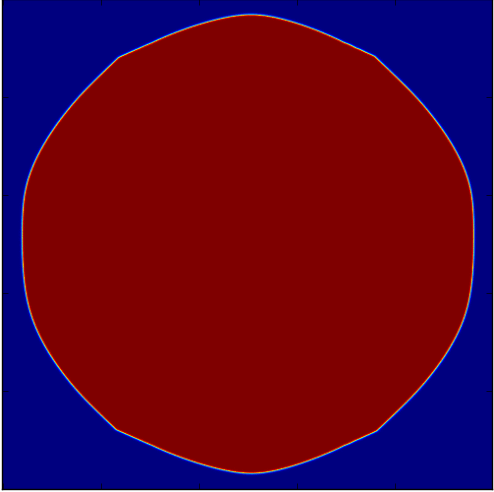
\includegraphics[width=0.15\textwidth]{../F-0.5-10.png}
  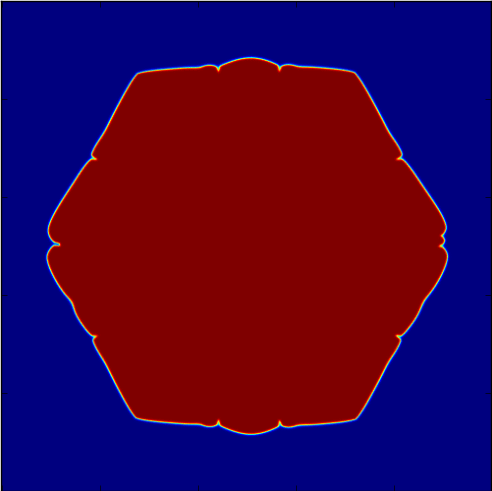
\includegraphics[width=0.15\textwidth]{../F-1.0-10.png}
  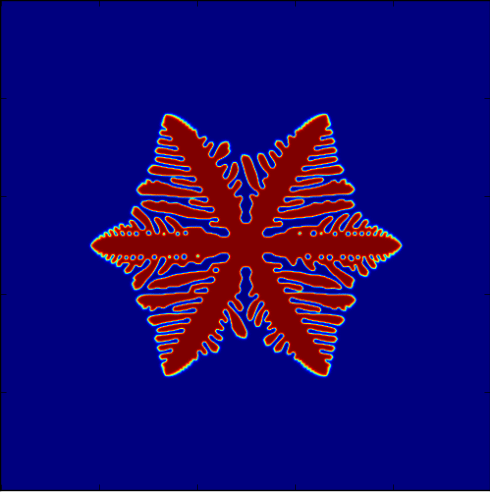
\includegraphics[width=0.15\textwidth]{../F-1.5-10.png}
  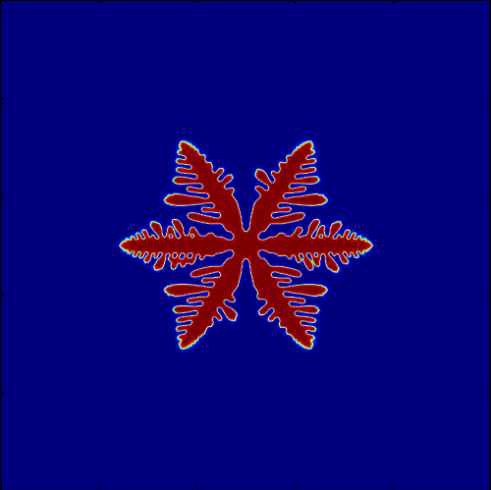
\includegraphics[width=0.15\textwidth]{../F-1.8-10.png}
  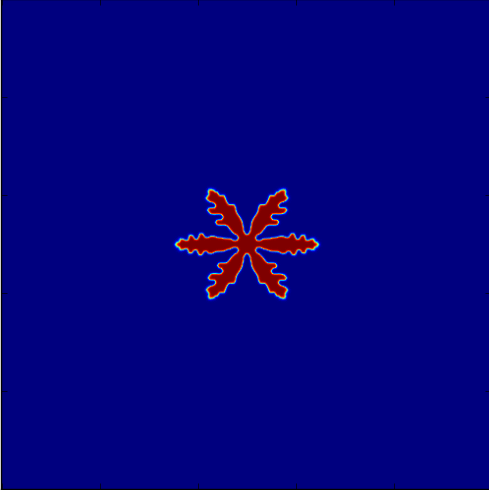
\includegraphics[width=0.15\textwidth]{../F-2.5-10.png}
  \caption{Effect of latent heat on crystal growth for the same parameters. Latent heat values of 0.5, 1.0, 1.5, 1.8 and 2.0 from left to right.}
  \label{fig:latent-heat}
\end{figure}

If latent heat is low, then little head is added to the system via crystallization and all angles of $\nabla\phi$ can crystallize. While the $\delta(\theta)$ term does add an energy cost to certain angles, we can see from Figure ($\ref{fig:latent-heat}.a$) that minimizing potential f, which heavily favors the solid phase at low temperatures, outweighs the cost of certain angles.\\

At higher values of K the opposite is true. When crystallization introduces lots of heat to the system, melting begins to take effect and we no longer see rampant crystal growth. We can assume that because size decreases with K, at higher temperatures our f is shifted to favor the liquid phase, so the magnitude of $\frac{\delta G}{\delta\phi}$ is lower, leading to slower growth. The reason anisotropy is more pronounced at high K is that at low K, the magnitude of potential f is much larger than the anisotropic interfacial width term, so anisotropy is less important. At temperatures closer to equilibrium f becomes much closer to zero, so anisotropy plays a larger role.\\

Figure ($\ref{fig:latent-heat}$) shows the temperature field for K=2.0. From this we can see that dimensionless temperature is fairly uniform around the boundary, at a value of about -0.9. At this value f still favors solidification, but it is less energetically favorable, which can explain why crystal formation is slower. \\

Figure ($\ref{fig:latent-heat-cold}$) shows the same information for K=0.8. Here we can see that at this lower value of K the bulk of the crystal is about $0.025$ degreeless temperature units colder than the K=2.0 crystal. This is a small amount, but it may be enough to explain why such rampant growth occurs at such a low value of K.\\

\begin{figure}[h!]
  \centering
  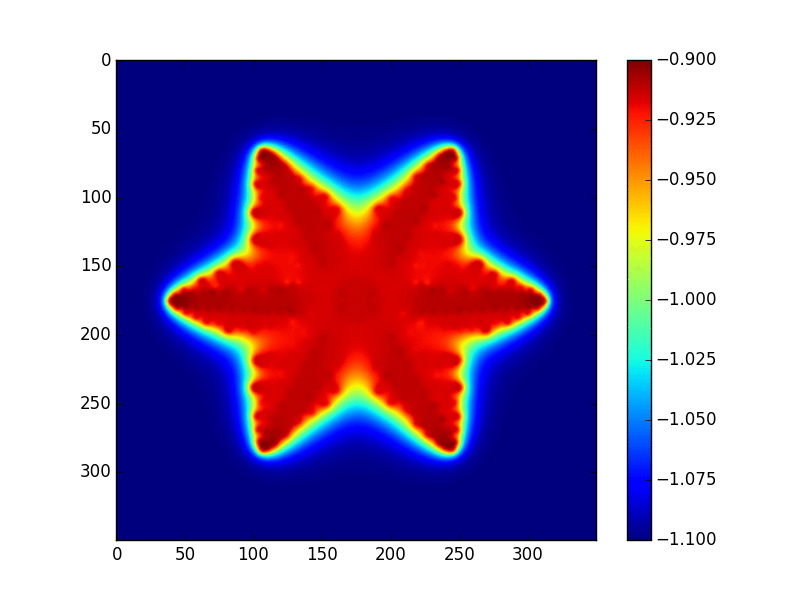
\includegraphics[width=0.45\textwidth]{../u-field-6.png}
  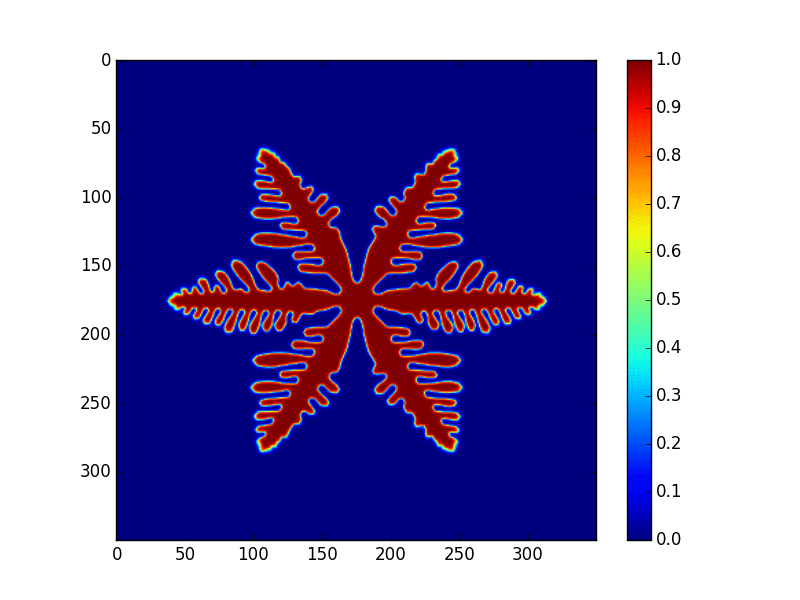
\includegraphics[width=0.45\textwidth]{../phi-field-6.png}
  \caption{Plots of both temperature and phi for a K=2.0 crystal growth.}
  \label{fig:latent-heat}
\end{figure}

\begin{figure}[h!]
  \centering
  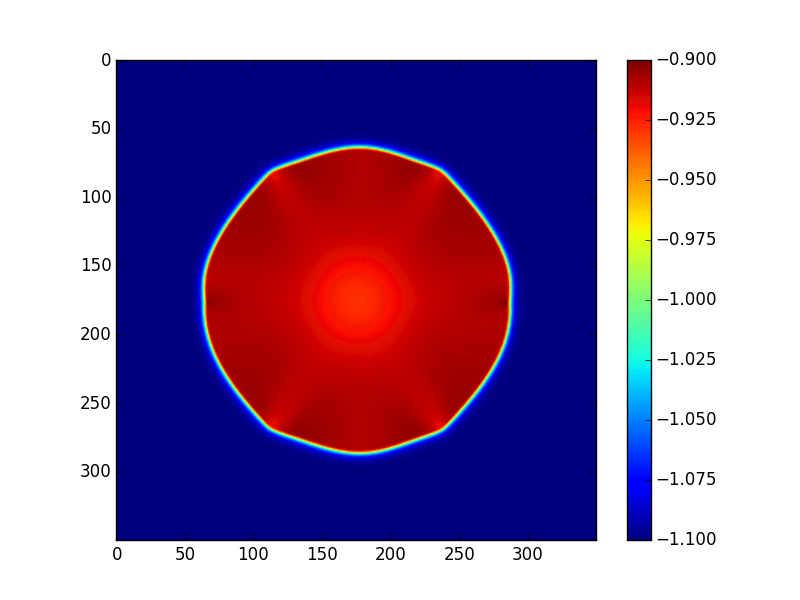
\includegraphics[width=0.45\textwidth]{../u-cold-field-3.png}
  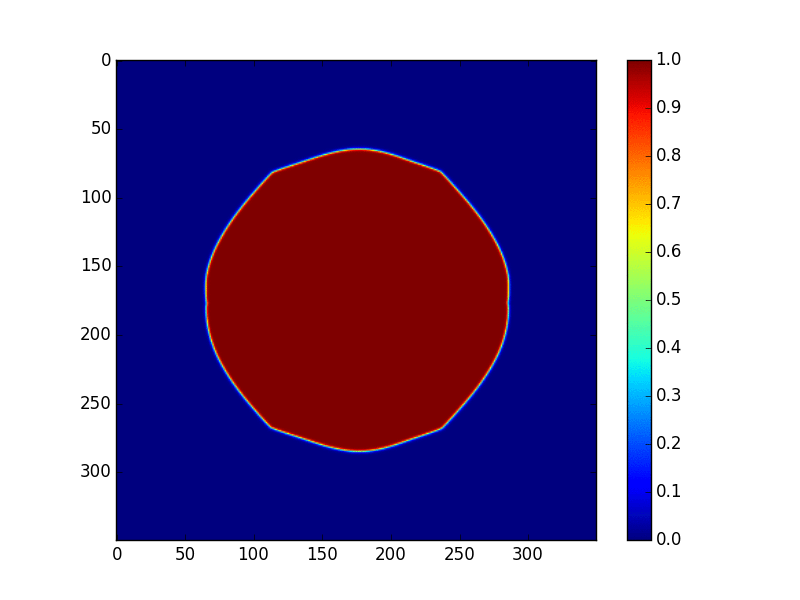
\includegraphics[width=0.45\textwidth]{../phi-cold-field-3.png}
  \caption{Plots of both temperature and phi for a K=0.8 crystal growth.}
  \label{fig:latent-heat-cold}
\end{figure}

\subsection{Anisotropy}
The original model used in Kobayashi [1] introduces anisotropy by making interface layer thickness $\delta$ a function of $\theta$, the angle between $\nabla\phi$ and the x-axis. This dependence is given by:\\

\begin{equation}
  \delta(\theta) = \delta_0(1 + \mu\cos(a_0(\theta-\theta_0)))
  \label{eq:kobayoshi-delta}
\end{equation}

where $\delta_0$ is the average layer width, $\mu$ is the strength of anisotropy and $\theta_0$ is the rotation of the crystal. Anisotropy is the most obvious parameter to change in this model. As expected, changing the modes in our $\delta(\theta)$ interface width changes the behavior based on circular initial conditions. Figure ($\ref{fig:anisotropy}$) shows crystal growth behavior for different anisotropies.\\

\begin{figure}[h!]
  \centering
  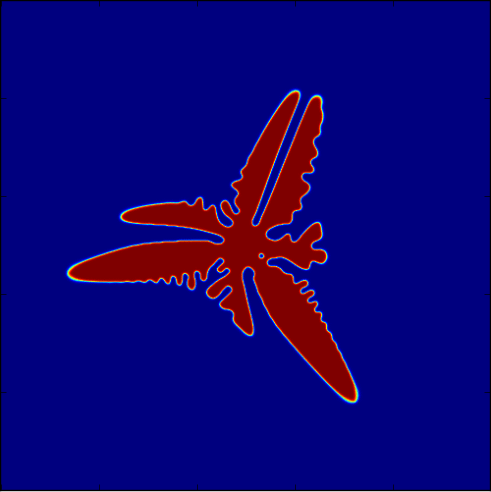
\includegraphics[width=0.15\textwidth]{../A-3-17.png}
  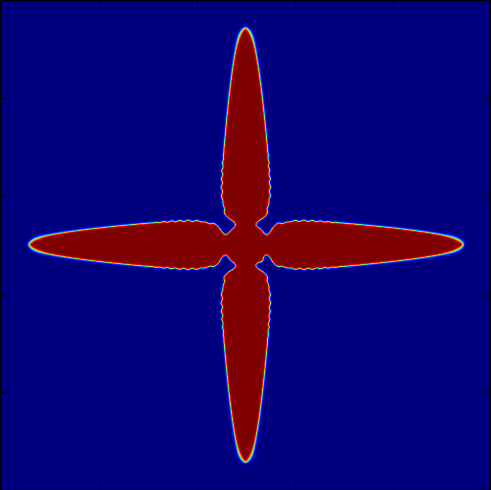
\includegraphics[width=0.15\textwidth]{../A-4-17.png}
  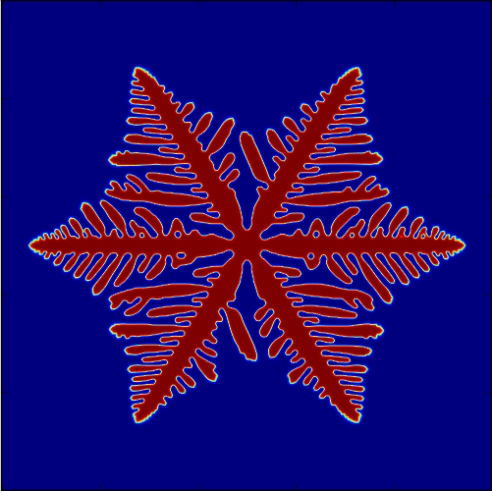
\includegraphics[width=0.15\textwidth]{../A-6-17.png}
  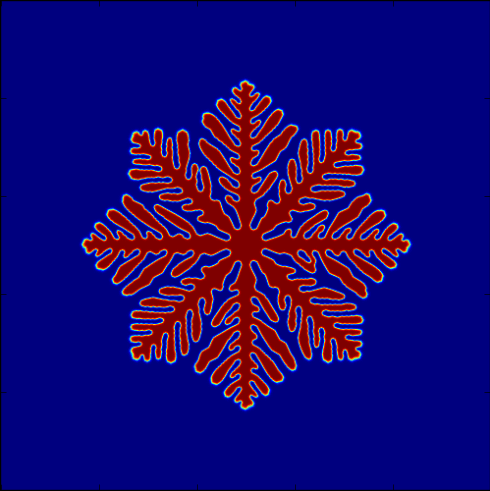
\includegraphics[width=0.15\textwidth]{../A-8-17.png}
  \caption{Effect of anisotropy on crystal formation. Anisotropy values of 3, 4, 6 and 8 from left to right.}
  \label{fig:anisotropy}
\end{figure}

In Figure ($\ref{fig:r-delta-4}$) we show how $\delta$ varies with $\theta$ and the effect this has on the resultant crystal. Figures ($\ref{fig:r-delta-3}$) and ($\ref{fig:r-delta-6}$) show the same effect for anisotropies of $6$ and $3$, respectively.\\

These plots carry a lot of explanatory power. The lighter regions represent the lowest values of $\delta$. The system tends to minimize free energy, and $\delta$ makes a positive contribution to the value of $G$. We can think of $\delta(\theta)$ as a cost function that makes certain angles of $\nabla\phi$ more expensive than others. If we look at Figure ($\ref{fig:r-delta-4}$.b), the plot for $a=4$, we can see that nearly all interface angles are at multiples of $\pi/2$. From Figure ($\ref{fig:r-delta-4}$.a) we can see that these are the least expensive angles. This same effect is seen by looking at Figure ($\ref{fig:r-delta-6}$), where $a=6$.\\

Interestingly, the effect is much less pronounced for Figure ($\ref{fig:r-delta-3}$) at $a=3$. By looking at Figure ($\ref{fig:r-delta-3}$.b) we see weaker anisotropy, or more angles in the crystal interface. This can be explained by looking at Equation ($\ref{eq:kobayoshi-delta}$). When anisotropy $a$ is low, angles near the minima are less expensive than they would be when anisotropy is high. This means that, while the system will still tend to maximize the lowest-cost angles, those near it will be more available, and thus the final crystal will have a wider variance in angles. The cosine function for lower modes is ``broader'', so the angles immediately near the minimum angles, which are dramatically more accessible to the system than those far from minima, are cheaper and therefore more represented.\\

\begin{figure}[h!]
  \centering
  \textbf{a. }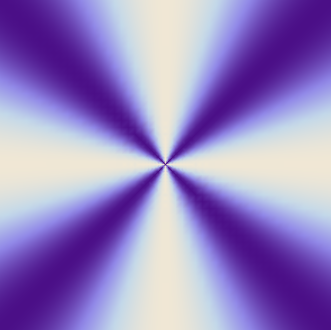
\includegraphics[width=0.25\textwidth]{../radial-anisotropy-4.png}
  \hspace{1cm}\textbf{b. }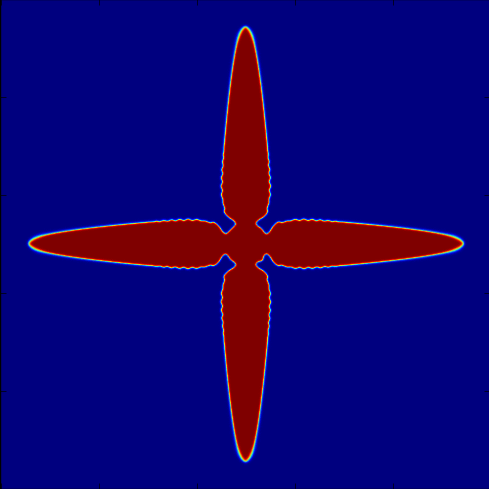
\includegraphics[width=0.25\textwidth]{../anis-4.png}
  \caption{\textbf{a.} Values of $\delta(\theta)$, where $\theta$ is the angular polar coordinate, translated from the rectangular coordinates centered in the middle, of points in the XY plane. Darker values correspond to larger values of $\delta$. \textbf{b.} The resulting crystal, plotted for the following parameters: $a=4$, $dx=0.0003$, $F=1.8$ and $t=0.2$.}
  \label{fig:r-delta-4}
\end{figure}

\begin{figure}[h!]
  \centering
  \textbf{a. }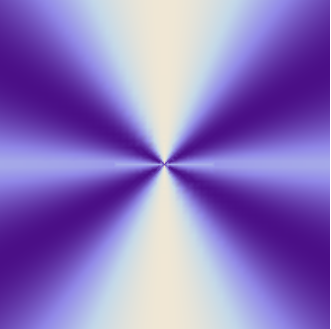
\includegraphics[width=0.25\textwidth]{../radial-anisotropy-3.png}
  \hspace{1cm}\textbf{b. }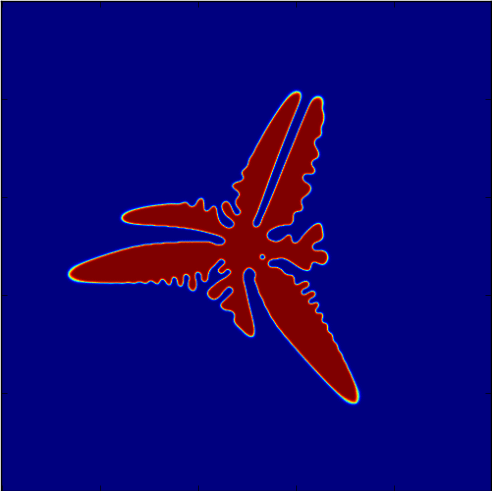
\includegraphics[width=0.25\textwidth]{../anis-3.png}
  \caption{$\delta$ and $\phi$, this time for $a=3$.}
  \label{fig:r-delta-3}
\end{figure}

\begin{figure}[h!]
  \centering
  \textbf{a. }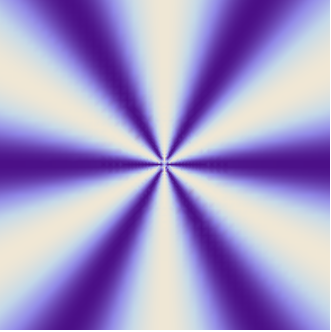
\includegraphics[width=0.25\textwidth]{../radial-anisotropy-6.png}
  \hspace{1cm}\textbf{b. }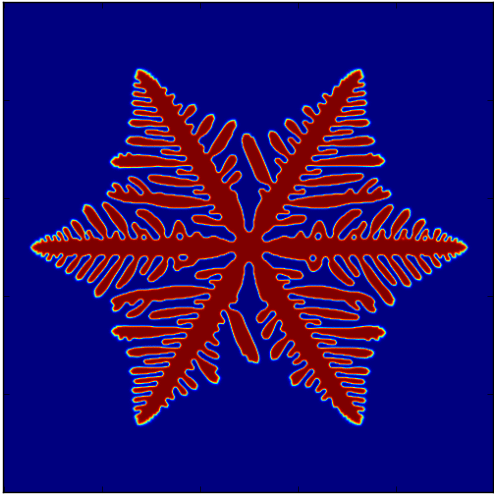
\includegraphics[width=0.25\textwidth]{../anis-6.png}
  \caption{$\delta$ and $\phi$, this time for $a=6$.}
  \label{fig:r-delta-6}
\end{figure}

\subsection{Layer Thickness}
Layer thickness has an interesting effect on the crystal growth. Increasing average layer thickness $\delta_0$ in Equation ($\ref{eq:kobayoshi-delta}$) effectively increases the magnitude of the anisotropy term in our free energy definition. We see this pattern reflected in Figure ($\ref{fig:delta}$). The highest $\delta_0$ crystal on the right seems to have the most ``anisotropy'' - it has the most offshoots, all travelling in the same direction (a minimum-energy angle in Figure ($\ref{fig:r-delta-6}$).a). The large non-phase regions at the edges of the main dendrites, the green regions between $\phi=0$ and $\phi=1$, can be explained by accepting that at high values of anisotropy the penalties of being at a non-phase $\phi$ value imposed by potential f are less important, since the anisotropy term has a larger magnitude. However, ``increased anisotropy'' doesn't fully describe the weirdness that arises in the $\delta_0 = 0.11$ crystal. It isn't intuitive why holes would show up in the middle of crystals. This is a yet unknown mystery of the $\delta_0$ parameter.\\

\begin{figure}[h!]
  \centering
  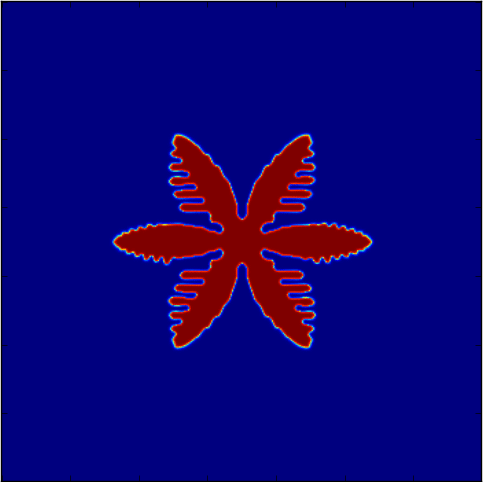
\includegraphics[width=0.2\textwidth]{../d-0.008-5.png}
  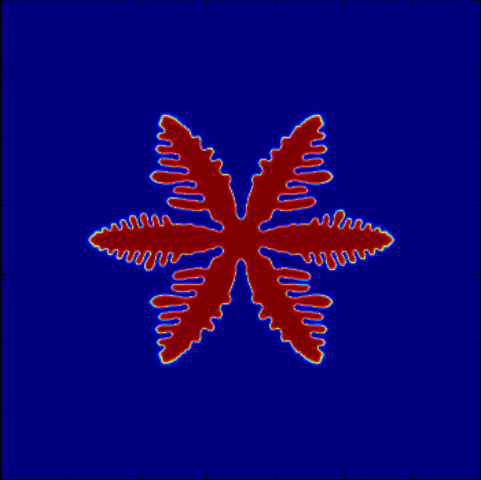
\includegraphics[width=0.2\textwidth]{../d-0.09-5.png}
  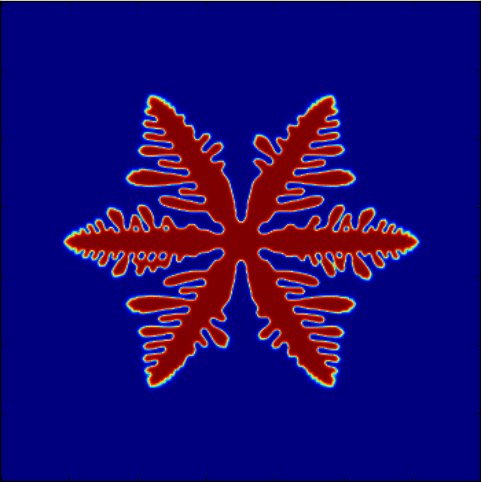
\includegraphics[width=0.2\textwidth]{../d-0.1-5.png}
  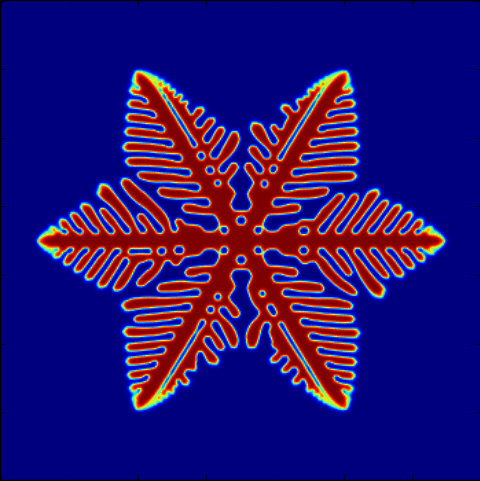
\includegraphics[width=0.2\textwidth]{../d-0.11-5.png}
  \caption{Effect of boundary width on crystal formation. $\delta$ values of 0.008, 0.009, 0.1 and 0.11 from left to right.}
  \label{fig:delta}
\end{figure}

\section{Variations on Model}
\subsection{Zhao Model}
The Zhao model, described in [2], is most notable because of its use of noise to simulate thermal fluctuations in the crystal formation. The evolution equation for $\phi$ is given by:

\begin{equation}
  \tau \frac{d\phi}{dt} = L_0\left(\frac{1}{T_M} - \frac{1}{F}\right)p'(\phi) - \frac{W_f}{\lambda^2}\frac{\partial^2\phi}{\partial\phi\partial T} + \frac{\epsilon_f^2}{T}\nabla^2\phi + f_0\\
\end{equation}

This model has some significant deviations from the original Kobayashi model. First, there is a latent heat term modifying the evolution of $\phi$. This is interesting because latent heat, and therefore the heat evolved from the crystal interface, has a direct impact on the change in $\phi$. This model does not use the same potential polynomial used in Kobayashi, so perhaps this is how the boundary movement is taken into account.\\

Another interesting aspect of this model is that, in an unfortunate symbol collision with the Sanal [3] crystal paper, $\epsilon_f$ is not the boundary width, but a constant. $W_f$ is the boundary width. This means that the all-important $\nabla^2\phi$ term is separated from the boundary width, which is very different from the traditional term found in Kobayashi:

\begin{equation}
  \frac{\delta^2(\nabla\phi)^2}{2}
\end{equation}

This suggests that perhaps the semi-unintuitive linking of the interface width term with $\nabla^2\phi$ is unnecessary.\\

The most important part of the Zhao model is that it introduces randomness into the deterministic Kobayashi model. The $f_0$ term on the right is a Gaussian-sampled zero-centered term which randomly speeds up or slows down crystal formation. The effects of this added randomness are shown in [2]. The crystals evolved with noise show more small dendrites shooting off the main ones, which makes sense. Small nucleations of new dendrites can be caused by the $f_0$ term which would otherwise never show up.\\

\subsection{LDA Model}
This is less a new model and more a limiting case of the Kobayashi model. When the discussed material is particularly inert, we can make the Local Density Approximation and discount the effects of surface tension. Thus, the only energy we need to worry about is our potential, which can be given by a simple polynomial, such as the equilibrium case $f_{eq} = (1-\phi^2)^2/4$, as given in Biben [4]. In the case of this model, already existing boundaries would solidify, but extra terms are needed to actually cause crystal formation.\\

In the section on latent heat we discussed how the magnitude of the phase potential vs surface tension (anisotropy) terms in our free energy definition changed the behavior. Figure ($\ref{fig:latent-heat}.a$) is an approximation to the LDA model. As we have argued, the potential term must outweigh the anisotropy term since we see little anisotropy in this crystal and rampant growth.\\

\section{Further Questions}
The major puzzle still present in this model is the reason for angular assymetry. It seems the model should be completely radially symmetric for all values of anisotropy. Figures $\ref{fig:r-delta-4}.a$, $\ref{fig:r-delta-3}.a$ and $\ref{fig:r-delta-6}.a$ are all angularly symmetric. While the angular plot for $a=3$ is less ``well-behaved'' than the even anisotropy plots, it is still symmetric. The more chaotic behavior of this plot may at least partially explain why the anisotropy-3 crystal is so much more strange-looking than the others, but it is not a complete explanation.\\

It is unlikely that the asymmetry comes from a defect in the simulation itself, since angular asymmetry can also be seen in Biben [4] and Shah [5]. It remains to be see what the source of this is.\\

\section{Reference}
\textbf{[1]} Kobayashi, R. (1993) Modeling and Numerical Simulations of Dendritic Crystal Growth. \textit{Physica D}, 63, 410-423. http://dx.doi.org/10.1016/0167-2789(93)90120-P\\
\textbf{[2]} Zhao, Y and Hou, H (2013). Simulation of Dendritic Crystal Growth of Pure Ni using the Phase-Field Model. \textit{Rev. Adv. Mater. Sci.}, 33, 246-250\\
\textbf{[3]} Sanal, R (2014). Numerical Simulation of Dendritic crystal growth using phase field method and investigating the effects of different physical parameter on the growth of the dendrite. UBid 50094548. Arxiv: http://arxiv.org/ftp/arxiv/papers/1412/1412.3197.pdf\\
\textbf{[4]} Biben, T. (2005) Phase-Field Models for Free-Boundary Problems. \textit{European Journal of Physics}, 26, 47-55. http://dx.doi.org/10.1088/0143-0807/26/5/S06\\
\textbf{[5]} Shah, A \textit{et. al} (2014). Numerical Simulation of Two-Dimensional Dendritic Growth Using Phase-Field Model. \textit{World Journal of Mechanics}, 128-136. http://dx.doi.org/10.4236/wjm.2014.45015
\end{document}
